\section{Évaluation}
\label{sec:evaluation}
  Pour valider notre approche, nous réalisons une première série d'évaluations
  visant à déterminer la configuration optimale de TopicRank. Nous comparons 
  ensuite TopicRank aux méthodes précédentes et analysons l'impact de chacune de
  nos contributions.

  \subsection{Cadre expérimental}
  \label{subsec:cadre_experimental}
    \subsubsection{Données de test}
    \label{subsubsec:donnees_de_test}
      \TODO{Quels types d'évaluations}
      Les collections de données présentées ci-dessous sont utilisées lors de
      toutes les évaluations. Afin de suivre \newcite{hassan2010conundrums} qui
      soulignent l'importance d'évaluer une méthode avec des collections de
      données aux configurations différentes pour mieux observer et comprendre
      son comportement, les collections de données utilisées ici diffèrent en
      termes de langue, nature, taille des documents et types d'annotateur
      (auteurs, lecteurs ou les deux).

      \textbf{DUC}~\cite{over2001duc} est une collection en anglais issue des
      données de la campagne d'évaluation DUC-2001. Cette campagne d'évaluation
      concerne les méthodes de résumé automatique, elle ne contient donc
      originellement pas d'annotations en termes-clés. Cependant, les 308
      articles journalistiques de la partie test de DUC-2001 ont été annotés par
      \newcite{wan2008expandrank}. Lors de nos expériences, nous utilisons ces
      308 documents.

      \textbf{SemEval}~\cite{kim2010semeval} est la collection en anglais
      fournie lors de la campagne d'évaluation SemEval-2010 pour la tâche
      d'extraction automatique de termes-clés. Cette collection contient 284
      articles scientifiques (conférences et ateliers) issus de la librairie
      numérique ACM. La collection est répartie en trois sous-ensembles, un
      ensemble de 40 documents d'essais, un ensemble de 144 documents
      d'entraînement et un ensemble de 100 documents de test. Lors de nos
      expériences, nous utilisons les 100 documents de l'ensemble de test. En ce
      qui concerne les termes-clés associés aux documents, ils correspondent à
      la combinaison de ceux donnés par les auteurs et des lecteurs.

      \textbf{WikiNews}\footnote{\url{https://github.com/adrien-bougouin/WikinewsKeyphraseCorpus}}
      est une collection de 100 articles journalistiques en français que nous
      avons extraits du site Web
      WikiNews\footnote{\url{http://fr.wikinews.org}} entre les mois de mai et
      décembre 2012. Chaque document est annoté par au moins trois étudiants,
      les termes-clés des différents étudiants sont groupés et les redondances
      lexicales sont automatiquement supprimées. \TODO{Détailler plus}

      \textbf{DEFT}~\cite{paroubek2012deft} est la collection fournie lors de la
      campagne d'évaluation DEFT-2012 pour la tâche d'extraction automatique de
      termes-clés. Celle-ci contient 234 documents en français issus de quatre
      revues de Sciences Humaines et Sociales. La collection est divisée en deux
      sous-ensembles, un ensemble d'entraînement contenant 141 documents et un
      ensemble de test contenant 93 documents. Lors de nos expériences, nous
      utilisons les 93 documents de l'ensemble de test. Seuls les termes-clés
      des auteurs sont disponibles pour cette collection.

      Le tableau~\ref{tab:donnees_de_test} donne les statistiques extraites des
      quatre collections de données présentées ci-dessus. Les données sont
      divisées en deux langues (anglais et français), avec pour chaque langue
      une collection de documents courts (articles journalistiques) et une
      collection de documents de plus grande taille (articles scientifiques). Il
      est aussi important de noter qu'en fonction du type d'annotateurs, le
      nombre de termes-clés associés varie, de même que le nombre de termes-clés
      n'apparaissant pas dans les documents.
      \begin{table}
        \centering
        \begin{tabular}{@{~}r@{~~}c@{~~}c@{~~}c@{~~}c@{~}}
          \toprule
          \textbf{Statistique} & \textbf{DUC} & \textbf{SemEval} & \textbf{WikiNews} & \textbf{DEFT}\\
          \midrule
          Langue & Anglais & Anglais & Français & Français\\
          Nature & Journalistique & Scientifique & Journalistique & Scientifique\\
          \multirow{3}{*}[.35em]{Annotateurs} & \multirow{3}{*}[.35em]{Lecteurs} & Auteurs & \multirow{3}{*}[.35em]{Lecteurs} & \multirow{3}{*}[.35em]{Auteurs}\\
          \addlinespace[-.7\defaultaddspace]
          & & \& & &\\
          \addlinespace[-.7\defaultaddspace]
          & & Lecteurs & &\\
          Documents & 308 & 100 & 100 & 93\\
          Mos/document & 900,7 & 5177,7 & 308,5 & 6839,4\\
          Termes-clés/document & 8,1 & 14,7 & 9,6 & 5,2\\
          Mots/termes-clés & 2,1 & 2,1 & 1,7 & 1,6\\
          Termes-clés manquants & 3,5\% & 22,1\% & 7,6\% & 21,1\% \\
          \bottomrule
        \end{tabular}
        \caption{Statistiques sur les données de test utilisées. En accord avec
                 l'évaluation effectuée lors de nos expériences, la proportion
                 de termes-clés manquant est déterminée sans tenir compte de la
                 flexions des mots. \TODO{Rmax}
                 \label{tab:donnees_de_test}}
      \end{table}

    \subsubsection{Prétraitement}
    \label{subsubsec:pretraitement}
      Chaque document des collections de données utilisées subit les mêmes
      prétraitements. Chaque document est tout d'abord segmenté en phrases, puis
      en mots et enfin étiqueté en parties du discours. La segmentation en mots
      est effectuée par le TreeBankWordTokenizer, disponible avec la librairie
      python NLTK~\cite[\textit{Natural Language ToolKit}]{bird2009nltk}, pour
      l'anglais et par l'outil Bonsai, du Bonsai PCFG-LA
      parser\footnote{\url{http://alpage.inria.fr/statgram/frdep/fr_stat_dep_parsing.html}},
      pour le français. Quant à l'étiquetage en parties du discours, il est
      réalisé avec le Stanford POS tagger~\cite{toutanova2003stanfordpostagger}
      pour l'anglais, et avec MElt~\cite{denis2009melt} pour le français. Tous
      ces outils sont utilisés avec leur configuration par défaut.

    \subsubsection{Mesures d'évaluation}
    \label{subsubsec:mesures_d_evaluation}
      Les performances des méthodes d'extraction de termes-clés sont exprimées
      en termes de précision (P), rappel (R) et f-score (f1-mesure, F). Afin de
      ne pas considérer fausse l'extraction d'une variante flexionnelle d'un
      terme-clé de référence, les opérations de comparaison sont effectuées à
      partir de la forme radicale des mots.

    \subsubsection{Méthodes de référence pour l'extraction de termes-clés}
    \label{subsubsec:systemes_de_reference_pour_l_extraction_de_termes_cles}
      % Comment les baselines sont-elles choisies ?
      Dans nos expérimentations, nous comparons TopicRank avec trois autres
      méthodes non-supervisées d'extraction automatique de termes-clés. Nous
      choisissons TextRank et SingleRank, les deux méthodes qui sont la
      fondation des méthodes à base de graphe, et la pondération TF-IDF. Cette
      dernière consiste à donner un score aux termes-clés candidats en faisant
      la somme des poids TF-IDF des mots qui les composent, puis à sélectionner
      ceux ayant le plus haut score. \TODO{Être clair sur pourquoi pas
      ExpandRank}

      % Quelles sont les particularités liées à notre implémentation ?
      Toutes les méthodes de référence sont implémentées par nous-même
      \TODO{Liens GitHub}. Lorsque
      celles-ci ont des parties communes avec TopicRank, elles bénéficient des
      mêmes composants. De plus, pour améliorer les résultats des méthodes de
      référence, leurs sorties sont filtrées afin de supprimer les termes-clés
      candidats dont les mots ont la même forme radicale que ceux d'un candidat
      mieux classé. Ce filtrage ne dégrade en rien les résultats et a pour effet
      de faire monter de nouveaux candidats dans le classement.

  \subsection{Analyse empirique de TopicRank}
  \label{subsection:configuration_empirique_de_topicrank}
    À ce stade des expérimentations, nous tentons de déterminer quels sont les
    paramètres optimaux pour TopicRank. En effet, TopicRank possède trois points
    de variabilités~: le seuil de groupement ($\zeta$), la stratégie de
    groupement (simple, complète ou moyenne) et la stratégie de sélection du
    terme-clé candidat le plus représentatif d'un sujet. Deux expériences sont
    réalisées, l'une pour déterminer la configuration de groupement optimale
    (variation du seuil $\zeta$ et de la stratégie de groupement) et l'autre
    pour déterminer la stratégie de sélection des termes-clés représentatifs.

%    \begin{table}
%      \centering
%      \begin{tabular}{@{~}r@{~~}c@{~~}c@{~~}c@{~~}c@{~~}c@{~~}c@{~~}c@{~~}c@{~~}c@{~~}c@{~~}c@{~~}c@{~}}
%        \toprule
%        \multirow{2}{*}[-2pt]{\textbf{Seuil $\boldsymbol{\zeta}$}} & \multicolumn{3}{c}{\textbf{DUC}} & \multicolumn{3}{c}{\textbf{SemEval}} & \multicolumn{3}{c}{\textbf{WikiNews}} & \multicolumn{3}{c}{\textbf{DEFT}}\\
%        \cmidrule(r){2-4}\cmidrule(r){5-7}\cmidrule(r){8-10}\cmidrule{11-13}
%        & P & R & F & P & R & F & P & R & F & P & R & F\\
%        \midrule
%        0,17 & 18.6 & 23.7 & 20.6 & 14.8 & 10.2 & 12.0 & 34.6 & 37.1 & 35.2 & 10.9 & 20.2 & 14.0\\
%        \addlinespace[.75\defaultaddspace]
%        0,25 & 17,7 & 22,6 & \textbf{19,6} & 14,9 & 10,3 & \textbf{12,1} & 35,0 & 37,5 & 35,6 & 11,7 & 21,7 & \textbf{15,1}\\
%        \addlinespace[.75\defaultaddspace]
%        0,33 & 17,2 & 22,1 & 19,1 & 13,0 & $~~$9,0 & 10,5 & 35,3 & 37,6 & \textbf{35,8} & 11,3 & 20,9 & 14,5\\
%        \addlinespace[.75\defaultaddspace]
%        0,50 & 13,6 & 17,8 & 15,2 & $~~$9,6 & $~~$6,7 & $~~$7,8 & 35,0 & 37,6 & 35,7 & 11,0 & 20,2 & 14,0\\
%        \addlinespace[.75\defaultaddspace]
%        0,67 & $~~$9.9 & 13.1 & 11.1 & $~~$10.5 & $~~$7.4 & $~~$8.6 & 35.0 & 37.0 & 35.4 & 11.0 & 20.0 & 14.0\\
%        \bottomrule
%      \end{tabular}
%      \caption{Résultats de l'extraction de 10 termes-clés, avec TopicRank, en
%               fonction de la valeur du seuil de similarité.
%               \label{tab:variation_du_seuil_de_similarite}}
%    \end{table}
%    \begin{table}
%      \centering
%      \begin{tabular}{@{~}r@{~~}c@{~~}c@{~~}c@{~~}c@{~~}c@{~~}c@{~~}c@{~~}c@{~~}c@{~~}c@{~~}c@{~~}c@{~}}
%        \toprule
%        \multirow{2}{*}[-2pt]{\textbf{Groupement}} & \multicolumn{3}{c}{\textbf{DUC}} & \multicolumn{3}{c}{\textbf{SemEval}} & \multicolumn{3}{c}{\textbf{WikiNews}} & \multicolumn{3}{c}{\textbf{DEFT}}\\
%        \cmidrule(r){2-4}\cmidrule(r){5-7}\cmidrule(r){8-10}\cmidrule{11-13}
%        & P & R & F & P & R & F & P & R & F & P & R & F\\
%        \midrule
%        Simple & 17,2 & 22,0 & 19,1 & 12,0 & $~~$8,4 & $~~$9,8 & 34,7 & 37,1 & 35,3 & 11,1 & 20,2 & 14,2\\
%        \addlinespace[.75\defaultaddspace]
%        Complet & 16,7 & 21,4 & 18,5 & $~~$3,7 & $~~$2,7 & $~~$3,1 & 34,0 & 36,3 & 34,6 & $~~$5,1 & $~~$9,6 & $~~$6,5\\
%        \addlinespace[.75\defaultaddspace]
%        Moyen & 17,7 & 22,6 & \textbf{19,6} & 14,9 & 10,3 & \textbf{12,1} & 35,0 & 37,5 & \textbf{35,6} & 11,7 & 21,7 & \textbf{15,1}\\
%        \bottomrule
%      \end{tabular}
%      \caption{Résultats de l'extraction de 10 termes-clés, avec TopicRank, en
%               fonction des différentes stratégies de regroupement.
%               \label{tab:comparaison_des_strategies_de_groupement}}
%    \end{table}
    \begin{figure}
      \centering
      \subfigure[DUC]{
        \begin{tikzpicture}
          \begin{axis}[axis lines=middle,
                       x=0.35\linewidth,
                       xtick={0.0, 0.2, ..., 1.2},
                       xmin=0.0,
                       xmax=1.05,
                       xlabel=$\zeta$,
                       y=0.003\textheight,
                       ytick={0, 10, ..., 40},
                       ymin=0,
                       ymax=42.5,
                       ylabel=F,
                       label style={anchor=south}]
            % simple
            \addplot[green!66, mark=x] coordinates{
              (0.05, 18.2)
              (0.10, 18.2)
              (0.15, 18.1)
              (0.20, 18.3)
              (0.25, 18.5)
              (0.30, 19.0)
              (0.35, 18.5)
              (0.40, 18.5)
              (0.45, 18.6)
              (0.50, 18.6)
              (0.55, 11.1)
              (0.60, 11.1)
              (0.65, 11.1)
              (0.70, 11.1)
              (0.75, 11.2)
              (0.80, 11.2)
              (0.85, 11.2)
              (0.90, 11.2)
              (0.95, 11.2)
              (1.00, 10.9)
            };
            % complet
            \addplot[cyan!66, mark=+] coordinates{
              (0.05, 19.7)
              (0.10, 19.7)
              (0.15, 19.5)
              (0.20, 19.2)
              (0.25, 19.1)
              (0.30, 18.1)
              (0.35, 15.2)
              (0.40, 15.2)
              (0.45, 15.1)
              (0.50, 15.1)
              (0.55, 11.0)
              (0.60, 11.0)
              (0.65, 11.0)
              (0.70, 11.1)
              (0.75, 11.2)
              (0.80, 11.2)
              (0.85, 11.2)
              (0.90, 11.2)
              (0.95, 11.2)
              (1.00, 10.9)
            };
            % moyen
            \addplot[red!66, mark=o] coordinates{
              (0.05, 21.0)
              (0.10, 21.4)
              (0.15, 21.0)
              (0.20, 20.1)
              (0.25, 19.6)
              (0.30, 19.4)
              (0.35, 18.4)
              (0.40, 17.0)
              (0.45, 15.4)
              (0.50, 15.2)
              (0.55, 11.1)
              (0.60, 11.0)
              (0.65, 11.0)
              (0.70, 11.1)
              (0.75, 11.2)
              (0.80, 11.2)
              (0.85, 11.2)
              (0.90, 11.2)
              (0.95, 11.2)
              (1.00, 11.2)
            };
            \draw ({axis cs:0.10,0}|-{rel axis cs:0,1}) -- ({axis cs:0.10,0}|-{rel axis cs:0,0}) [color=red!66];
            \node at (axis cs:0.10,40) [color=red!66, anchor=west] {\tiny{0.10}};
          \end{axis}
        \end{tikzpicture}
      }
      \subfigure[SemEval]{
        \begin{tikzpicture}
          \begin{axis}[axis lines=middle,
                       x=0.35\linewidth,
                       xtick={0.0, 0.2, ..., 1.2},
                       xmin=0.0,
                       xmax=1.05,
                       xlabel=$\zeta$,
                       y=0.003\textheight,
                       ytick={0, 10, ..., 40},
                       ymin=0,
                       ymax=42.5,
                       ylabel=F,
                       label style={anchor=south}]
            % simple
            \addplot[green!66, mark=x] coordinates{
              (0.05, 3.1)
              (0.10, 3.1)
              (0.15, 3.1)
              (0.20, 3.1)
              (0.25, 3.1)
              (0.30, 3.5)
              (0.35, 5.5)
              (0.40, 5.5)
              (0.45, 5.7)
              (0.50, 5.7)
              (0.55, 7.3)
              (0.60, 7.3)
              (0.65, 7.2)
              (0.70, 8.6)
              (0.75, 8.4)
              (0.80, 8.4)
              (0.85, 8.4)
              (0.90, 8.4)
              (0.95, 8.4)
              (1.00, 8.5)
            };
            % complet
            \addplot[cyan!66, mark=+] coordinates{
              (0.05, 11.5)
              (0.10, 11.5)
              (0.15, 11.3)
              (0.20, 11.0)
              (0.25, 9.8)
              (0.30, 8.3)
              (0.35, 7.8)
              (0.40, 7.8)
              (0.45, 7.8)
              (0.50, 7.8)
              (0.55, 7.6)
              (0.60, 7.6)
              (0.65, 7.6)
              (0.70, 8.6)
              (0.75, 8.4)
              (0.80, 8.4)
              (0.85, 8.4)
              (0.90, 8.4)
              (0.95, 8.4)
              (1.00, 8.5)
            };
            % moyen
            \addplot[red!66, mark=o] coordinates{
              (0.05, 11.0)
              (0.10, 10.7)
              (0.15, 11.5)
              (0.20, 12.3)
              (0.25, 12.1)
              (0.30, 11.2)
              (0.35, 9.6)
              (0.40, 8.7)
              (0.45, 7.8)
              (0.50, 7.8)
              (0.55, 7.1)
              (0.60, 7.3)
              (0.65, 7.6)
              (0.70, 8.6)
              (0.75, 8.4)
              (0.80, 8.4)
              (0.85, 8.4)
              (0.90, 8.4)
              (0.95, 8.4)
              (1.00, 8.4)
            };
            \draw ({axis cs:0.20,0}|-{rel axis cs:0,1}) -- ({axis cs:0.20,0}|-{rel axis cs:0,0}) [color=red!66];
            \node at (axis cs:0.20,40) [color=red!66, anchor=west] {\tiny{0.20}};
            \legend{Simple, Complet, Moyen}
          \end{axis}
        \end{tikzpicture}
      }
      \subfigure[WikiNews]{
        \begin{tikzpicture}
          \begin{axis}[axis lines=middle,
                       x=0.35\linewidth,
                       xtick={0.0, 0.2, ..., 1.2},
                       xmin=0.0,
                       xmax=1.05,
                       xlabel=$\zeta$,
                       y=0.003\textheight,
                       ytick={0, 10, ..., 40},
                       ymin=0,
                       ymax=42.5,
                       ylabel=F,
                       label style={anchor=south}]
            % simple
            \addplot[green!66, mark=x] coordinates{
              (0.05, 34.2)
              (0.10, 34.2)
              (0.15, 34.2)
              (0.20, 34.3)
              (0.25, 34.6)
              (0.30, 35.2)
              (0.35, 35.7)
              (0.40, 35.7)
              (0.45, 35.7)
              (0.50, 35.7)
              (0.55, 35.1)
              (0.60, 35.1)
              (0.65, 35.1)
              (0.70, 35.4)
              (0.75, 35.4)
              (0.80, 35.4)
              (0.85, 35.4)
              (0.90, 35.4)
              (0.95, 35.4)
              (1.00, 34.9)
            };
            % complet
            \addplot[cyan!66, mark=+] coordinates{
              (0.05, 35.2)
              (0.10, 35.2)
              (0.15, 35.2)
              (0.20, 35.3)
              (0.25, 35.3)
              (0.30, 35.8)
              (0.35, 35.7)
              (0.40, 35.7)
              (0.45, 35.7)
              (0.50, 35.7)
              (0.55, 35.1)
              (0.60, 35.1)
              (0.65, 35.1)
              (0.70, 35.4)
              (0.75, 35.4)
              (0.80, 35.4)
              (0.85, 35.4)
              (0.90, 35.4)
              (0.95, 35.4)
              (1.00, 34.9)
            };
            % moyen
            \addplot[red!66, mark=o] coordinates{
              (0.05, 34.4)
              (0.10, 34.8)
              (0.15, 35.0)
              (0.20, 35.4)
              (0.25, 35.6)
              (0.30, 35.7)
              (0.35, 35.8)
              (0.40, 35.8)
              (0.45, 35.7)
              (0.50, 35.7)
              (0.55, 35.1)
              (0.60, 35.1)
              (0.65, 35.1)
              (0.70, 35.4)
              (0.75, 35.4)
              (0.80, 35.4)
              (0.85, 35.4)
              (0.90, 35.4)
              (0.95, 35.4)
              (1.00, 35.4)
            };
            \draw ({axis cs:0.35,0}|-{rel axis cs:0,1}) -- ({axis cs:0.35,0}|-{rel axis cs:0,0}) [color=red!66];
            \node at (axis cs:0.35,40) [color=red!66, anchor=west] {\tiny{0.35}};
          \end{axis}
        \end{tikzpicture}
      }
      \subfigure[DEFT]{
        \begin{tikzpicture}
          \begin{axis}[axis lines=middle,
                       x=0.35\linewidth,
                       xtick={0.0, 0.2, ..., 1.2},
                       xmin=0.0,
                       xmax=1.05,
                       xlabel=$\zeta$,
                       y=0.003\textheight,
                       ytick={0, 10, ..., 40},
                       ymin=0,
                       ymax=42.5,
                       ylabel=F,
                       label style={anchor=south}]
            % simple
            \addplot[green!66, mark=x] coordinates{
              (0.05, 6.4)
              (0.10, 6.4)
              (0.15, 6.4)
              (0.20, 6.5)
              (0.25, 6.5)
              (0.30, 6.5)
              (0.35, 8.3)
              (0.40, 8.3)
              (0.45, 8.3)
              (0.50, 8.3)
              (0.55, 13.6)
              (0.60, 13.6)
              (0.65, 13.6)
              (0.70, 14.0)
              (0.75, 14.0)
              (0.80, 14.0)
              (0.85, 14.0)
              (0.90, 14.0)
              (0.95, 14.0)
              (1.00, 13.4)
            };
            % complet
            \addplot[cyan!66, mark=+] coordinates{
              (0.05, 14.3)
              (0.10, 14.3)
              (0.15, 14.3)
              (0.20, 14.3)
              (0.25, 14.2)
              (0.30, 13.9)
              (0.35, 13.9)
              (0.40, 13.9)
              (0.45, 14.0)
              (0.50, 14.0)
              (0.55, 13.6)
              (0.60, 13.6)
              (0.65, 13.6)
              (0.70, 14.0)
              (0.75, 14.0)
              (0.80, 14.0)
              (0.85, 14.0)
              (0.90, 14.0)
              (0.95, 14.0)
              (1.00, 13.4)
            };
            % moyen
            \addplot[red!66, mark=o] coordinates{
              (0.05, 12.8)
              (0.10, 13.1)
              (0.15, 13.6)
              (0.20, 14.5)
              (0.25, 15.1)
              (0.30, 14.8)
              (0.35, 14.6)
              (0.40, 14.2)
              (0.45, 14.3)
              (0.50, 14.0)
              (0.55, 13.4)
              (0.60, 13.6)
              (0.65, 13.6)
              (0.70, 14.0)
              (0.75, 14.0)
              (0.80, 14.0)
              (0.85, 14.0)
              (0.90, 14.0)
              (0.95, 14.0)
              (1.00, 13.4)
            };
            \draw ({axis cs:0.25,0}|-{rel axis cs:0,1}) -- ({axis cs:0.25,0}|-{rel axis cs:0,0}) [color=red!66];
            \node at (axis cs:0.25,40) [color=red!66, anchor=west] {\tiny{0.25}};
          \end{axis}
        \end{tikzpicture}
      }
      \caption{Résultats de l'extraction de 10 termes-clés, avec TopicRank, en
               fonction de la stratégie de regroupement et de la valeur du seuil
               de similarité $\zeta$.
               \label{fig:variation_du_seuil_de_similarite}}
    \end{figure}

    % Variation du seuil de similarité et de la stratégie de groupement
    La figure~\ref{fig:variation_du_seuil_de_similarite} présente les résultats
    de TopicRank lorsque nous faisons varier le seuil $\zeta$ avec un pas de
    0,05 pour toutes les stratégies de groupement. La stratégie de sélection
    d'un terme-clé par sujet utilisée est celle qui consiste à sélectionner le
    candidat qui apparaît en premier dans le document pour chaque sujet.
    % Quelle analyse peut-on faire à partir des courbes ?
    Globalement, chaque stratégie de groupement a un comportement qui lui est
    propre jusqu'à un certain point de convergence lorsque $\zeta$ vaut 0,55.
    Avec la stratégie simple, les résultats s'améliorent lorsque le seuil
    $\zeta$ augmente. Du fait qu'elle ne prenne en compte que la similarité
    maximale entre deux candidats de deux groupes, cette stratégie à tendance à
    trop grouper et donc à créer des groupes contenant parfois plusieurs sujets.
    L'augmentation du seuil $\zeta$ a pour effet de restreindre cette tendance
    et la qualité du groupement s'améliore. En opposition, la stratégie
    complète, qui a le fonctionnement inverse, voie ses résultats se dégrader
    lorsque $\zeta$ augmente. Finalement, la stratégie moyenne, qui agit en tant
    que compromis, semble moins sensible aux variations de $\zeta$. Nous
    observons tout de même une dégradation des résultats jusqu'au point de
    convergence. Ce point de convergence correspond au moment où les groupes
    sont majoritairement composés de variantes flexionnelles, de variantes
    dérivationnelles où de candidats dont ceux contenant le plus de mots
    incluent les autres (par exemple, le sujet qui ne contient que \og nouvelles
    églises~\fg, \og nouvelles églises indépendantes protestantes~\fg,
    \og nouvelle église indépendante~\fg\ et \og nouvelles églises
    indépendantes~\fg\ avec le groupement moyen et $\zeta=\text{0,55}$ contient
    en plus \og églises évangéliques~\fg, ainsi que d'autres, lorsque $\zeta$
    est plus faible).
    % Quels sont les paramètres utilisés ?
    Après observation des résultats de cette expérience, le seuil $\zeta$ est
    fixé à 0,25 pour toutes les expériences suivantes. De même, la stratégie de
    groupement utilisée dans la suite est la stratégie moyenne.

    La figure~\ref{fig:variation_de_la_selection_des_candidats} présente les
    résultats obtenus avec TopicRank et les différentes stratégies de sélection
    d'un terme-clé candidat par sujet. Ceux-ci confirment ce qui est dit dans la
    section~\ref{sec:extraction_de_termes_cles_avec_topicrank} concernant le
    bien fondé de la sélection des candidats les plus fréquents ou des
    centroïdes. Ces dernières stratégies ont, en effet, tendance à sélectionner
    des concepts inhérents qui jouent un rôle crucial lors du groupement, mais
    qui ne sont pas les candidats les plus représentatifs des sujets.
%    \begin{table}
%      \centering
%      \begin{tabular}{@{~}r@{~~}c@{~~}c@{~~}c@{~~}c@{~~}c@{~~}c@{~~}c@{~~}c@{~~}c@{~~}c@{~~}c@{~~}c@{~}}
%        \toprule
%        \multirow{2}{*}[-2pt]{\textbf{Sélection}} & \multicolumn{3}{c}{\textbf{DUC}} & \multicolumn{3}{c}{\textbf{SemEval}} & \multicolumn{3}{c}{\textbf{WikiNews}} & \multicolumn{3}{c}{\textbf{DEFT}}\\
%        \cmidrule(r){2-4}\cmidrule(r){5-7}\cmidrule(r){8-10}\cmidrule{11-13}
%        & P & R & F & P & R & F & P & R & F & P & R & F\\
%        \midrule
%        Position & 17,7 & 22,6 & \underline{19,6} & 14,9 & 10,3 & \underline{12,1} & 35,0 & 37,5 & \underline{35,6} & 11,7 & 21,7 & \underline{15,1}\\
%        Fréquence & 15,1 & 18,7 & 16,5 & $~~$1,7 & $~~$1,2 & $~~$1,4 & 25,7 & 27,6 & 26,2 & $~~$1,9 & $~~$3,8 & $~~$2,5\\
%        Centroïde & 13,0 & 16,3 & 14,3 & $~~$1,9 & $~~$1,2 & $~~$1,5 & 28,1 & 29,9 & 28,5 & $~~$2,6 & $~~$5,0 & $~~$3,4\\
%        \midrule
%        Borne haute & 37,1 & 41,1 & 38,6 & 37,6 & 25,8 & \textbf{30,3} & 42,5 & 44,8 & \textbf{42,9} & 14,9 & 28,0 & \textbf{19,3}\\
%        \bottomrule
%      \end{tabular}
%      \caption{Résultats de l'extraction de 10 termes-clés, avec TopicRank, en
%               fonction des différentes sélections de termes-clés candidats par
%               sujets.
%               \label{tab:variation_de_la_selection_des_candidats}}
%    \end{table}
    \begin{figure}
      \centering
      \begin{tikzpicture}
        \begin{axis}[axis lines=left,
                     symbolic x coords={DUC, SemEval, WikiNews, DEFT},
                     xtick=data,
                     enlarge x limits=0.25,
                     x=.19\linewidth,
                     nodes near coords,
                     nodes near coords align={vertical},
                     every node near coord/.append style={font=\tiny},
                     y=0.004\textheight,
                     ytick={0, 10, ..., 50},
                     ymin=0,
                     ymax=52.5,
                     ybar=4pt,
                     ylabel=F,
                     ylabel style={at={(ticklabel* cs:1)},
                                   anchor=south,
                                   rotate=270}]%,
                     %legend style={at={(0.5,-0.15)},
                     %              anchor=north,
                     %              legend columns=-1}]
          % fréquence
          \addplot[green!66,
                   pattern=north west lines,
                   pattern color=green!40] coordinates{
            (DUC,       16.5)
            (SemEval,   1.4)
            (WikiNews,  26.2)
            (DEFT,      2.5)
          };
          % centroïde
          \addplot[black!66,
                   pattern=north east lines,
                   pattern color=black!40] coordinates{
            (DUC,       14.3)
            (SemEval,   1.5)
            (WikiNews,  25.5)
            (DEFT,      3.4)
          };
          % position
          \addplot[cyan!66,
                   pattern=horizontal lines,
                   pattern color=cyan!40] coordinates{
            (DUC,       19.6)
            (SemEval,   12.1)
            (WikiNews,  35.6)
            (DEFT,      15.1)
          };
          % borne haute
          \addplot[red!66,fill=red!40] coordinates{
            (DUC,       38.6)
            (SemEval,   30.3)
            (WikiNews,  42.9)
            (DEFT,      19.3)
          };

          \legend{Fréquence, Centroïde, Position, Borne haute}
        \end{axis}
      \end{tikzpicture}
      \caption{Résultats de l'extraction de 10 termes-clés, avec TopicRank, en
               fonction des différentes sélections de termes-clés candidats par
               sujet.
               \label{fig:variation_de_la_selection_des_candidats}}
    \end{figure}
    Bien que la sélection à partir de la première position des candidats donne
    des résultats satisfaisants, nous remarquons qu'il existe encore une marge
    de progression importante. Les valeurs indiquées par la borne haute
    représentent les résultats qui pourraient être obtenus avec un oracle. Pour
    chacun des sujets les plus importants, l'oracle sélectionne toujours un
    candidat positif, s'il y en a un. La marge de progression allant de 4,2 à
    19,0 points de f-score est encourageante pour de futurs travaux.

  \subsection{Comparaison de TopicRank avec l'existant}
  \label{subsec:comparaison_de_topicrank_avec_l_existant}
    % Que représente le tableau ?
    Le tableau~\ref{tab:resultats_globaux} montre les performances de TopicRank
    comparées à celles des trois méthodes de référence.
    % Que peut-on dire globalement ?
    Globalement, TopicRank donne de meilleurs résultats que les méthodes de
    référence utilisées.
    % Que peut-on dire de plus ? (analyse plus approfondie)
    Comparée à la méthode TF-IDF, TopicRank donne de meilleurs résultats pour
    SemEval, WikiNews et DEFT. Cette supériorité vis-à-vis de TF-IDF est
    importante à noter, car cette méthode obtient de bons résultats en tirant
    parti de statistiques extraites de documents supplémentaires (apprentissage
    non-supervisé), alors que TopicRank n'utilise que le document à analyser.
    Comparée aux autres méthodes à base de graphe, TopicRank donne des
    résultats significativement meilleurs pour SemEval, WikiNews et DEFT. Ceci
    confirme donc que le groupement des candidats permet de rassembler des
    informations améliorant la précision de l'ordonnancement. En ce qui concerne
    DUC, notre méthode est toujours significativement meilleure que TextRank,
    mais elle ne l'est pas vis-à-vis des autres méthodes. Aux vues de la borne
    haute de la figure~\ref{fig:variation_de_la_selection_des_candidats}, l'une
    des raisons pour lesquelles les résultats sont moins bons pour DUC est que
    la stratégie de sélection des candidats les plus représentatifs des sujets
    n'est pas adaptée. En effet, la différence avec la borne haute est de 19,0
    points de f-score. Une analyse plus approfondie des différents apports de
    TopicRank peut aussi donner une piste sur les raisons de ces moins bons
    résultats.
    \begin{table}
      \centering
      \begin{tabular}{@{~}r@{~~}c@{~~}c@{~~}c@{~~}c@{~~}c@{~~}c@{~~}c@{~~}c@{~~}c@{~~}c@{~~}c@{~~}c@{~}}
        \toprule
        \multirow{2}{*}[-2pt]{\textbf{Méthode}} & \multicolumn{3}{c}{\textbf{DUC}} & \multicolumn{3}{c}{\textbf{SemEval}} & \multicolumn{3}{c}{\textbf{WikiNews}} & \multicolumn{3}{c}{\textbf{DEFT}}\\
        \cmidrule(r){2-4}\cmidrule(r){5-7}\cmidrule(r){8-10}\cmidrule{11-13}
        & P & R & F & P & R & F & P & R & F & P & R & F\\
        \midrule
        TF-IDF & \textbf{23,8} & \textbf{30,7} & \textbf{26,4} & 13,2 & $~~$8,9 & 10,5$^{~}$ & 33,9 & 35,9 & 34,3$^{~}$ & 10,3 & 19,1 & 13,2$^{~}$\\
        TextRank & $~~$4,9 & $~~$5,4 & $~~$5,0 & $~~$7,9 & $~~$4,5 & $~~$5,6$^{~}$ & $~~$9,3 & $~~$8,3 & $~~$8,6$^{~}$ & $~~$4,9 & $~~$7,1 & $~~$5,7$^{~}$\\
        SingleRank & 22,3 & 28,4 & 24,6 & $~~$4,6 & $~~$3,2 & $~~$3,7$^{~}$ & 19,4 & 20,7 & 19,7$^{~}$ & $~~$4,5 & $~~$9,0 & $~~$5,9$^{~}$\\
        TopicRank & 17,7 & 22,6 & 19,6 & \textbf{14,9} & \textbf{10,3} & \textbf{12,1}$^\dagger$ & \textbf{35,0} & \textbf{37,5} & \textbf{35,6}$^\dagger$ & \textbf{11,7} & \textbf{21,7} & \textbf{15,1}$^\dagger$\\
        \bottomrule
      \end{tabular}
      \caption{Résultats de l'extraction de 10 termes-clés avec TF-IDF,
               TextRank, SingleRank et TopicRank. $\dagger$ indique une
               amélioration significative de TopicRank vis-à-vis de TextRank et
               SingleRank, à 0,001 pour le t-test de Student.
               \label{tab:resultats_globaux}}
    \end{table}

    \begin{table}
      \centering
      \begin{tabular}{@{~}r@{~~}c@{~~}c@{~~}c@{~~}c@{~~}c@{~~}c@{~~}c@{~~}c@{~~}c@{~~}c@{~~}c@{~~}c@{~}}
        \toprule
        \multirow{2}{*}[-2pt]{\textbf{Méthode}} & \multicolumn{3}{c}{\textbf{DUC}} & \multicolumn{3}{c}{\textbf{SemEval}} & \multicolumn{3}{c}{\textbf{WikiNews}} & \multicolumn{3}{c}{\textbf{DEFT}}\\
        \cmidrule(r){2-4}\cmidrule(r){5-7}\cmidrule(r){8-10}\cmidrule{11-13}
        & P & R & F & P & R & F & P & R & F & P & R & F\\
        \midrule
        SingleRank & \textbf{22,3} & \textbf{28,4} & \textbf{24,6} & $~~$4,6 & $~~$3,2 & $~~$3,7$^{~}$ & 19,4 & 20,7 & 19,7$^{~}$ & $~~$4,5 & $~~$9,0 & $~~$5,9$^{~}$\\
        +complet & 22,2 & 28,1 & 24,5 & $~~$5,5 & $~~$3,8 & $~~$4,4$^{~}$ & 20,0 & 21,4 & 20,3${~}$ & $~~$4,4 & $~~$9,0 & $~~$5,8$^{~}$\\
        +candidats & 10,0 & 13,1 & 11,2 & $~~$9,6 & $~~$7,0 & $~~$8,0$^\dagger$ & 28,6 & 30,1 & 28,9$^\dagger$ & 10,5 & 19,7 & 13,5$^\dagger$\\
        +sujets & 18,4 & 23,6 & 20,5 & 14,7 & 10,2 & 11,9$^\dagger$ & 31,0 & 32,8 & 31,4$^\dagger$ & 11,5 & 21,4 & 14,8$^\dagger$\\
        TopicRank & 17,7 & 22,6 & 19,6 & \textbf{14,9} & \textbf{10,3} & \textbf{12,1}$^\dagger$ & \textbf{35,0} & \textbf{37,5} & \textbf{35,6}$^\dagger$ & \textbf{11,7} & \textbf{21,7} & \textbf{15,1}$^\dagger$\\
        \bottomrule
      \end{tabular}
      \caption{Résultats de l'extraction de 10 termes-clés avec chacune des
               contributions de TopicRank appliquées séparément à SingleRank.
               $\dagger$ indique une amélioration significative vis-à-vis de
               SingleRank, à 0,001 pour le t-test de Student.
               \label{tab:evaluation_individuelle_des_ameliorations}}
    \end{table}

    \TODO{Bien montrer que SingleRank +toutes les contribution est égale à
    TopicRank}
    Dans le but de confirmer la pertinence de tous les apports de TopicRank,
    nous réalisons une expérience supplémentaire dans laquelle la méthode
    SingleRank est modifiée de sorte qu'elle ordonne les mots avec un graphe
    complet, qu'elle ordonne les termes-clés candidats à la place des mots ou
    qu'elle ordonne les sujets à la place des mots (respectivement +complet,
    +candidats et +sujets). Les résultats de ces trois variantes de SingleRank
    sont présentés dans le
    tableau~\ref{tab:evaluation_individuelle_des_ameliorations}. Globalement,
    l'usage des termes-clés candidats, ou des sujets, induit une amélioration
    significative des performances de SingleRank, avec une amélioration plus
    importante en utilisant les sujets. Cela confirme la pertinence d'ordonner
    directement les candidats, plutôt que les mots. De plus, le groupement des
    candidats représentant le même sujet améliore la précision de
    l'ordonnancement grâce à la mutualisation des relations qu'ils entretiennent
    avec les candidats représentant d'autres sujets. L'usage d'un graphe
    complet, quant à lui, n'améliore pas significativement les résultats de
    SingleRank. Ceux-ci sont compétitifs vis-à-vis de ceux obtenus en
    construisant un graphe de co-occurrences. Nous pensons tout de même que
    l'usage du graphe complet est à privilégier afin d'éviter la fenêtre de
    co-occurrences.
    
    En ce qui concerne la collection DUC, le
    tableau~\ref{tab:evaluation_individuelle_des_ameliorations} montre une perte
    de performance induite par la construction du graphe avec les termes-clés
    candidats. Cette perte de performance s'explique par le fait qu'il y a, dans
    les documents de DUC, peu de répétition des candidats, notamment ceux de
    plus d'un mot. Le graphe créé contient alors moins de relations de
    co-occurrences que lorsque les n\oe{}uds sont les mots du document et est
    donc moins précis pour l'ordonnancement. Ceci se confirme avec la
    figure~\ref{fig:variation_de_la_selection_des_candidats} qui montre que
    l'extraction des candidats les plus fréquents, pour chaque sujet de DUC,
    donne des résultats proches de ceux obtenus avec l'extraction des candidats
    apparaissant en premier dans le document.

  \subsection{Analyse des sujets détectés}
  \label{subsec:analyse_des_sujets_générés}
    \TODO{S'intéresser aussi au termes-clés non détectés?}
    \TODO{Attention aux exemples foireux}

    Dans cette section, nous analysons les groupements en sujets effectués par
    TopicRank et tentons de déterminer quelles sont les causes principales
    d'erreurs. Notre langue maternelle étant le français et les documents de
    WikiNews étant de trop courts pour que nous puissions observer un nombre
    significatif de groupements en sujets, nos observations ci-dessous sont
    faites à partir des documents de la collection DEFT. Nous distinguons deux
    types d'erreurs~: celles qui sont liées à du bruit introduit dans les
    groupes et celles qui sont liées à des candidats ayant des propriétés
    particulières.

    Nous observons des erreurs liées à l'extraction des termes-clés candidats.
    Lors de l'extraction des candidats, certaines unités textuelles sont
    extraites à cause d'erreurs dans l'étiquetage grammatical. Ces erreurs
    concernent principalement la détection des prépositions composées et la
    détection des participes. Dans le document \textit{as\_2006\_014935ar}, nous
    observons par exemple que \og pays dits~\fg\ est un terme-clé candidats, car
    le participe passé \og dits~\fg\ est considéré comme un adjectif dans la
    phrase \og [\dots] elles ne cessent de se développer à travers le monde et
    particulièrement dans les \underline{pays dits} ``du sud'' [\dots]~\fg.

    En ce qui concerne les candidats ayant des propriétés particulières, nous
    observons tout d'abord de nombreuses erreurs lorsque les groupements sont
    déclenchés par un adjectif. Ce sont particulièrement les expansions
    nominales s'effectuant à gauche qui sont la source d'erreurs (\og même
    langue~\fg\ groupé avec \og même représentation~\fg, \og grands
    traits~\fg\ groupé avec \og grande ignorance~\fg, etc.). Parmi les
    expansions nominales s'effectuant à droite, les adjectifs relationnels sont
    moins sujets aux erreurs que les autres adjectifs. Notons tout de même que
    lorsque ces adjectifs ont attraits au contexte général du document, ils sont
    très fréquemment utilisés et beaucoup de candidats les contenant sont
    groupés par erreur. Ainsi, dans le document \textit{as\_2002\_000707ar} qui
    examine l'organisation du dialogue politique économique entre les membres de
    la commission européenne, les termes-clés candidats \og forces
    économiques~\fg, \og type économique~\fg, \og délabrement économique~\fg\ et
    \og économies postsocialistes~\fg\ sont groupés par erreur, car ils
    partagent tous l'adjectif \og économique~\fg. Outre ces groupements erronés,
    nous observons aussi de mauvais groupements lorsque les candidats ne
    contiennent que très peu de mots. En effet, pour les candidats de deux mots,
    il ne suffit que d'un seul mot en commun pour les grouper. Ces candidats
    étant très fréquents, ils sont la cause de nombreuses erreurs.

%    En plus, nous observons des erreurs liées à l'utilisation des radicaux lors
%    du calcul de la similarité de Jaccard. Des candidats tels que \og empire
%    ottoman~\fg\ et \og définition empirique~\fg\ sont alors groupés du fait que
%    les mots \og empire~\fg\ et \og empirique~\fg\ partagent le même radical
%    (\og empir~\fg) selon la méthode de \newcite{porter1980suffixstripping} .

